\documentclass[a4paper]{article}
\usepackage[utf8]{inputenc}
\usepackage[T1]{fontenc}
\usepackage[left=3cm, right=3cm]{geometry}
\usepackage{graphicx}
\usepackage{listings}
\usepackage{latexsym}
\usepackage{amsfonts}
\usepackage[hidelinks]{hyperref}
\usepackage{amssymb}
\usepackage{wasysym}
\usepackage[dvipsnames]{xcolor}

\newcommand{\command}[1]{\subsection{#1}}


\lstset{
  language=C++,
  basicstyle=\small\ttfamily,
  keywordstyle=\color{ForestGreen}\ttfamily,
  identifierstyle=\ttfamily,
  commentstyle=\color{gray}\ttfamily,
  stringstyle=\color{Purple}\ttfamily,
  showstringspaces=false,
  emph=[1]{std,vector,string,Eigen,VectorXd,bool,double,char,void},
  emphstyle=[1]{\color{blue}},
}


\begin{document}

\begin{center}
  \begin{huge}
    \textbf{The Figure Class\\}
  \end{huge}
  Basic plotting in C++
\end{center}
  
\vspace*{3cm}
  \tableofcontents
\vspace*{\fill}

\newpage
\newgeometry{bottom=2cm, left=3cm, right=3cm}
\section{Installation}

Follow the steps in the \texttt{INSTALL} file. \\
In the directory of the \texttt{CMakeLists.txt} do: \\ \\
Under Linux/Mac OS: \\
\texttt{
\indent   \$ mkdir build \\
\indent   \$ cd build \\
\indent   \$ cmake .. \\
\indent   \$ sudo make install \\ \\
}
Under Windows: \\
\indent    - open a terminal with administrator rights \\
\indent    - do the same as above but without the \texttt{sudo} \\ \\
%
This installation requires CMake (\url{https://cmake.org/download/}). 
The ``manual'' way of installing it is described in \texttt{INSTALL}.

\subsection{Opening example}

This short example code will show, how the Figure class can be used.
\begin{lstlisting}
int main()
{
  std::vector<double> x(10), y(10);
  for (int i = 1; i <= 10; ++i){ 
    x[i] = i; y[i] = std::exp(std::cos(0.2*i));
  }
  Eigen::VectorXd u = Eigen::VectorXd::LinSpaced(500, 1, 10),
                  v = ( (0.2*u.array()).cos().exp() ).matrix();
  Figure fig;
  fig.plot(x, y, " +r", "Sample Data");
  fig.plot(u, v, "b", "Function");
  fig.legend();
  fig.save("plot.eps");
  return 0;
}
\end{lstlisting}

\begin{figure}[h]
  \centering
  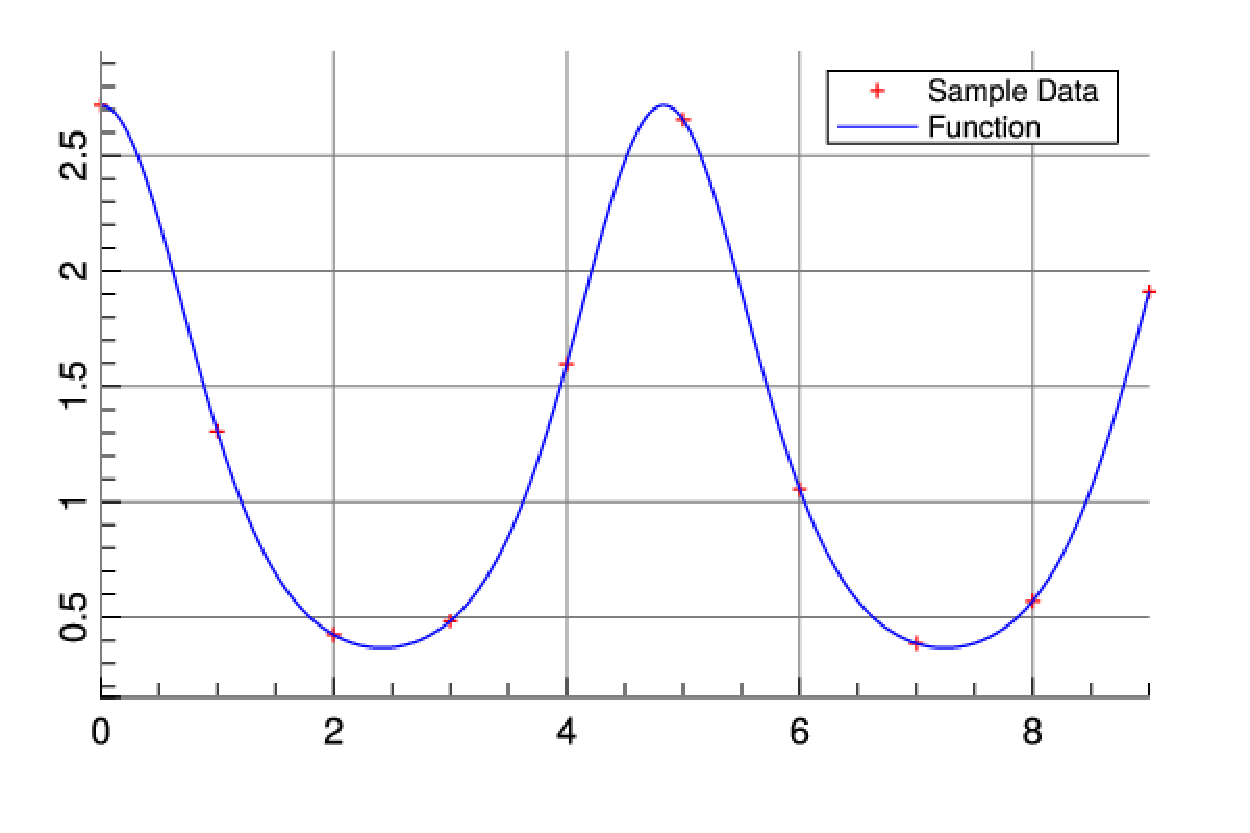
\includegraphics[width=0.7\textwidth]{opening-example.pdf}
  \thispagestyle{empty}
\end{figure}

\restoregeometry
\newpage
\section{Commands}

\command{grid}

\textbf{Definition:}
\begin{lstlisting}
void grid( const bool on = true, 
           const std::string gridType = "-", 
           const std::string gridCol = "h" )
\end{lstlisting}
%
\textbf{Restrictions:} None. \\ \\
%
\textbf{Examples:}
\begin{lstlisting}
  Figure fig;
  fig.plot(x, y, "r");
  fig.grid(false); // unset grid
  fig.save("plot.eps");

  Figure fig;
  fig.plot(x, y, "r");
  fig.grid(true, "!", "b"); // blue fine mesh
  fig.save("plot.eps");
\end{lstlisting}

\command{xlabel}

\textbf{Definition:}
\begin{lstlisting}
void xlabel( const char* label, 
             const double pos = 0 )
\end{lstlisting}
%
\textbf{Restrictions:} If \texttt{setlog} is called \texttt{xlabel} should be called beforehand. \\ \\
%
\textbf{Examples:}
\begin{lstlisting}
  Figure fig;
  fig.plot(x, y, "+g"); // '+g' equals matlab/python '+-g'
  fig.xlabel("Linear x axis");
  fig.save("plot.eps");

  Figure fig;
  fig.setlog(true, true);
  fig.plot(x, y, "+g");
  fig.xlabel("Logarithmic x axis"); // Not good - should be called before 'setlog'
  fig.save("plot.eps");

  Figure fig;
  fig.xlabel("Logarithmix x axis"); // Good
  fig.setlog(true, true);
  fig.plot(x, y, "+g");
  fig.save("plot.eps");
\end{lstlisting}

\newpage
\command{ylabel}

\textbf{Definition:}
\begin{lstlisting}
void ylabel( const char* label, 
             const double pos = 0 )
\end{lstlisting}
%
\textbf{Restrictions:} If \texttt{setlog} is called \texttt{ylabel} should be called beforehand. \\ \\
%
\textbf{Examples:} See \texttt{xlabel}.

\command{legend}

\textbf{Definition:}
\begin{lstlisting}
void legend( const double xPos = 1, 
             const double yPos = 1 )
\end{lstlisting}
%
\textbf{Restrictions:} None. 

\command{setlog}

\textbf{Definition:}
\begin{lstlisting}
void setlog( const bool logx = true, 
             const bool logy = true )
\end{lstlisting}
%
\textbf{Restrictions:} All plots will use the latest \texttt{setlog} options or default if none have been set. \\ \\
%
\textbf{Examples:}
\begin{lstlisting}
  Figure fig;
  fig.setlog(true, false); // -> semilogx
  fig.plot(x0, y0, "b"); 
  fig.setlog(false, true); // -> semilogy
  fig.plot(x1, y1, "r");
  fig.setlog(true, true); // -> loglog
  fig.plot(x2, y2, "g");
  fig.save("plot.eps"); // ATTENTION: all plots will have been plotted in loglog-scale 

  Figure fig;
  fig.plot(x, y, "b");
  fig.save("plot.eps"); // -> default (= linear) scaling
\end{lstlisting}


\command{plot} 

\textbf{Definition:} 
\begin{lstlisting}
template <typename yVector>
void plot( const yVector y, 
           const std::string style, 
           const char* legend = 0 )
\end{lstlisting}
\newpage

\begin{lstlisting}
template <typename xVector, typename yVector>
void plot( const xVector x, 
           const yVector y, 
           const std::string style, 
           const char* legend = 0 ) 
\end{lstlisting}
\textbf{Restrictions:} \texttt{xVector} and \texttt{yVector} must have a \texttt{size()} method, which returns the size of the vector 
and a \texttt{data()} method, which returns a pointer to the first element in the vector. \\
Furthermore \texttt{x} and \texttt{y} must have same length. Also note that the \texttt{style}-argument is required! \\ \\
%
\textbf{Examples:}
\begin{lstlisting}
  Figure fig;
  fig.plot(x, y, "b");
  fig.save("data.eps");

  Figure fig;
  fig.plot(x, y); // Not OK - style missing
  fig.save("data.eps");

  Figure fig;
  fig.plot(x, y, " *r", "Data w/ red dots"); // ' *r' equals matlab/python 'r*'
  fig.save("data.eps");
\end{lstlisting}

\command{fplot}

\textbf{Definition:}
\begin{lstlisting}
void fplot( const std::string function,
            const std::string style,
            const char* legend = 0 )
\end{lstlisting}
\textbf{Restrictions:} None. \\ \\
%
\textbf{Examples:}
\begin{lstlisting}
  Figure fig;
  fig.fplot("3*x\^2 + 4.5/x + exp(x)", "b");
  fig.fplot("exp(cos(pi*x))","r","some periodic function");
  fig.ranges(0.5, 2, 0, 5); // be sure to set ranges for fplot!
  fig.save("plot.eps");

  Figure fig;
  fig.plot(x, y, "b", "Benchmark");
  fig.fplot("x\^2", "k;", "\\ O(x\^2)");
  // here we don't set the ranges as it uses the range given by the x,y data
  // and we use fplot to draw a reference line (O(x\^2))
  fig.save("runtimes.eps"); 
\end{lstlisting}

\newpage
\command{ranges}

\textbf{Definition:}
\begin{lstlisting}
void ranges( const double xMin, 
             const double xMax, 
             const double yMin, 
             const double yMax )
\end{lstlisting}
%
\textbf{Restrictions:} xMin $<$ xMax, yMin $<$ yMax and ranges must be $>$ 0 for axis in logarithmic scale. \\ \\
%
\textbf{Examples:}
\begin{lstlisting}
  Figure fig;
  fig.ranges(-1,1,-1,1);
  fig.plot(x, y, "b");

  Figure fig;
  fig.plot(x, y, "b");
  fig.ranges(0, 2.3, 4, 5); // ranges can be called before or after 'plot'

  Figure fig;
  fig.ranges(-1, 1, 0, 5);
  fig.setlog(true, true); // will run but MathGL will throw a warning 
  fig.plot(x, y, "b");
\end{lstlisting}

\command{save}

\textbf{Definition:}
\begin{lstlisting}
void save( const char* file )
\end{lstlisting}
%
\textbf{Restrictions:} The filename \textit{must} end on \texttt{.eps}! \\ \\
%
\textbf{Examples:}
\begin{lstlisting}
  Figure fig;
  fig.save("plot.eps"); // OK
\end{lstlisting}
\begin{lstlisting}
  Figure fig;
  fig.save("plot.png"); // Not OK - Only eps-format supported!
\end{lstlisting}

\command{title}

\textbf{Definition:}
\begin{lstlisting}
void title( const char* text )
\end{lstlisting}
%
\textbf{Restrictions:} None.

\section{Line characteristics}

\begin{minipage}{3cm}
  Linecolors\footnote{
  Upper-case letters will give a darker version of the lower-case version.
  }:\\ \\
  \begin{tabular}{l|c}
    \textcolor{blue}{blue} & \texttt{b} \\
    \textcolor{green}{green} & \texttt{g} \\
    \textcolor{red}{red} & \texttt{r} \\
    \textcolor{cyan}{cyan} & \texttt{c} \\
    \textcolor{magenta}{magenta} & \texttt{m} \\
    \textcolor{yellow}{yellow} & \texttt{y} \\
    \textcolor[gray]{0.5}{gray} & \texttt{h} \\
    \textcolor{SeaGreen}{green-blue} & \texttt{l} \\
    \textcolor{RoyalBlue}{sky-blue} & \texttt{n} \\
    \textcolor{orange}{orange} & \texttt{q} \\
    \textcolor{LimeGreen}{green-yellow} & \texttt{e} \\
    \textcolor{CadetBlue}{blue-violet} & \texttt{u} \\
    \textcolor{purple}{purple} & \texttt{p}
  \end{tabular}
\end{minipage}
\hfill
\begin{minipage}{4cm}
  Linestyles:\\ \\
  \begin{tabular}{l|c}
    none & \\
    solid & \texttt{-} \\
    dashed & \texttt{;} \\
    small dashed & \texttt{=} \\
    long dashed & \texttt{|} \\
    dotted & \texttt{:} \\
    dash-dotted & \texttt{j} \\
    small dash-dotted & \texttt{i} 
  \end{tabular}
  None is used as follows: \\
  \texttt{" r*"} gives red stars w/o any lines
\end{minipage}
\hfill
\begin{minipage}{2cm}
  Linemarkers:\\ \\
  \begin{tabular}{l|c}
    + & \texttt{+} \\
    o & \texttt{o} \\
    $\diamond$ & \texttt{d} \\
    $\cdot$ & \texttt{.} \\
    $\triangle$ & \texttt{\^{}} \\
    $\nabla$ &\texttt{v} \\
    $\lhd$ & \texttt{<} \\
    $\rhd$ & \texttt{>} \\
    $\odot$ & \texttt{\#.} \\
    $\boxplus$ & \texttt{\#+} \\
    $\boxtimes$ & \texttt{\#x} 
  \end{tabular}
\end{minipage}



\end{document}
